% ==============================================================================
% TCC - Nome do Aluno
% Capítulo 1 - Introdução
% ==============================================================================
\chapter{Introdução}
\label{sec-intro}
Na computação muitas aplicações necessitam considerar um conjunto um conjunto de conexões entre dados e uso de algoritmos nesses dados para poder responder perguntad como, se existe um caminho entre um objeto a outro seguindo por essas conexões, qual a menor dinstância entre eles ou ainda quantos objetos podemos alcançar a partir de um determinado ponto. Para modelar tais situações, utilizamos um tipo abstrato chamado grafo \cite{ziviani2004projeto}.

\begin{figure}[H]
\centering
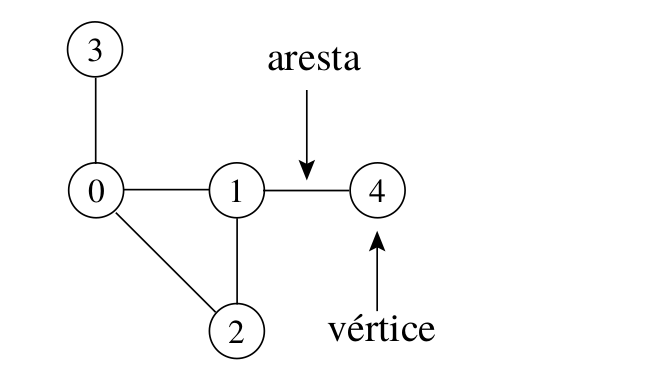
\includegraphics[width=.65\textwidth]{figuras/grafo-exemplo} 
\caption{Exemplo de um grafo.}
\label{fig-intro-exemplografo}
\end{figure}

Um problema clássico da literatura envolvendo grafos é o cálculo de caminho mínimo \cite{moura2010estudo}. Nele desejamos obter o menor caminho entre dois pontos específicos do grafo representado. A sua modelagem é feita representando as arestas com determinados pesos que podem significar o tempo decorrente entre executar tarefas, o custo de transmitir informações entre locais, quantidades específicas a serem transportadas entre um local e outro e etc \cite{drozdek2012data}. 

Dentre as modelagens realizadas para resolver o problema do caminho mínimo, uma que é abordada é a definição do menor caminho entre dois pontos geográficos tendo como aplicação prática o uso por softwares do tipo GPS. Nela representamos as interseções das ruas, caminhos ou rodovias como o vértices do grafo e as distâncias entre essas interseções (as próprias ruas, caminhos ou rodovias) como as arestas e tendo seus respectivos pesos como sendo a distâncias entre essas interseções.

A figura X mostra o exemplo desta modelagem abordada [a ser colocado ainda professora].

A motivação deste trabalho é o estudo dos algoritmos de menor caminho em grafos, desde os clássicos como o algoritmo de Dijkstra \cite{dijkstra1959note} até algoritmos mais recentes propostos como o Anytime Dynamic Search A* (AD*) \cite{likhachev2008anytime}. Tem por  objetivo verificar o desempenho e a eficácia destes algoritmos, averiguar o impacto que as estruturas de dados utilizadas para resolver o problema causam e analisar quais situações os algoritmos estudados melhor se aplicam.

\section{Revisão bibliográfica e trabalhos correlatos}
\label{sec-intro-correlatos}
O algoritmo de Dijkstra é amplamente difundido na literatura, sendo que é utilizado como base para o estudo desse algoritmo os livros de \citeonline{cormen2009introduction} e \citeonline{drozdek2012data}, em que abordam a descrição do algoritmo, estruturas de dados e a análise computacional das mesmas.

Para o algoritmo busca A*, será tido como base o uso do livro de \citeonline{russell1995modern} e \citeonline{likhachev2008anytime} que o cita e desenvolve seus algorimtos (ARA* e AD*) baseando-se naquele.

Já para os algoritmos ARA* e AD*, será utilizado o artigo que o propôs \cite{likhachev2008anytime}, e o estudo desses algoritmos realizados por \citeonline{moura2010estudo}.

O trabalho de \citeonline{larkin2014back} analisa o uso de diversas estrutura de dados como fila de prioridades e seus respectivos impactos, constatado diferenças entre a proposta teórica dessas estruturas e a aplicação prática.
\section{Metodologia de pesquisa}
\label{sec-intro-metodologia}
Para a realização do estudo a que este trabalho propõe, será implementado os algoritmos a serem estudados na linguagem Java, versão 1.8.0\_131. Os testes a serem realizados e as instâncias utilizadas estão descritos no capítulo \ref{sec-testes}. A configuração do computador em que será submetido os testes está descrito na tabela \ref{tbl-intro-configuracaomaquina}.

\begin{table}[H]
\centering
\caption{Configuração da máquina onde será realizado os testes computacionais.}
\label{tbl-intro-configuracaomaquina}
\begin{adjustbox}{max width=\textwidth}
\begin{tabular}{|c|c|}
\hline
Sistema Operacional & Linux Mint  18.2  Sonya 64-bit            \\ \hline
Processador         & Intel Core i5-2430M @ 2.40 GHz. Cache 6MB \\ \hline
Memória             & 4.0 GB                                    \\ \hline
Compilador          & Java 1.8.0\_131                           \\ \hline
\end{tabular}
\end{adjustbox}
\end{table}

\section{Organização dos capítulos}
\label{sec-intro-organizaocao}
Este trabalho está estruturado da seguinte forma:
\begin{description}
\item[Capítulo \ref{sec-dijkstra}:] Apresenta a descrição do algoritmo clássico de Dijkstra, as versões implementadas baseadas em estrutura de dados diferentes e suas respectivas descrições;
\item[Capítulo \ref{sec-aestrela}:] Apresenta a descrição do algoritmo busca A*, sua diferença em relação ao Dijkstra e uma descrição do uso da estratégia de heurísticas e como elas são classificadas;
\item[Capítulo \ref{sec-dinamicos}:] Apresenta a descrição dos algoritmos ARA* e AD*, a estratégia de heurística inflada e uma breve descrição de grafos dinâmicos, nos quais o algoritmo AD* se aplica;
\item[Capítulo \ref{sec-testes}:] Apresenta a descrição dos testes realizados, seus respectivos resultados e uma análise desses para cada algoritmo abordado;
\item[Capítulo \ref{sec-conclusao}:] Traz a conclusão geral deste trabalho e possíveis trabalhos futuros.
\end{description}